\chapter{Results}
\label{ch:results}

\section{Reproduction of the Detection Pipeline on UK Biobank}
\label{sec:results-reproduction}

Applying the reproduced pipeline (Section~\ref{sec:reproduction}) to the full set of UK Biobank
carotid ultrasound acquisitions yielded detections for 179{,}611 images from 20{,}014
participants. At the image level, 76.4\,\% of images contained no detection, 20.6\,\% one,
2.8\,\% two and 0.2\,\% three (Table~\ref{tab:plaque-counts}). Automated main-axis selection
retained 42{,}954 images from 19{,}778 participants; among these, 32{,}163 images carried no
detection, 9{,}318 one, 1{,}373 two and 100 three.

Aggregated to participant level, 8{,}504 of 19{,}778 participants (43.0\,\%) were classified as
plaque-positive. \textcite{omarov2024deep} report carotid plaques in 45\,\% of the cohort. Given
that main-axis selection was reimplemented independently and retains approximately 11\,\% more
images per participant than the original selection, this agreement to within two percentage
points indicates that the pipeline was reproduced faithfully at the level of the derived
phenotype, not merely at the level of the processed image count.

The prevalence is likewise consistent with the 41.9\,\% observed in the smaller proteomics
sub-cohort (Section~\ref{subsec:results-phase1a}), indicating that restriction to participants
with proteomics data did not appreciably shift the phenotype distribution.

\begin{table}[H]
\centering
\caption[Image-level plaque counts]{Distribution of detections per image before and after
automated main-axis selection.}
\label{tab:plaque-counts}
\begin{tabular}{lrrrr}
\hline
Detections per image & 0 & 1 & 2 & 3 \\
\hline
All images ($n=179{,}611$)        & 137{,}210 & 36{,}955 & 5{,}093 & 353 \\
Main-axis images ($n=42{,}954$)   & 32{,}163  & 9{,}318  & 1{,}373 & 100 \\
\hline
\end{tabular}
\end{table}

\section{Phase 1A: Proteomics Association Analysis}
\label{sec:results-phase1}

\subsection{Proteomics Dataset Overview}
The UK Biobank Olink proteomics panel comprised 2{,}923 proteins measured across 52{,}998 samples
(154{,}966{,}152 individual values in total), with an overall missingness of 10.3\,\%
(Table~\ref{tab:proteomics-missingness}). Missingness was unevenly distributed across
samples: while the median per-sample missingness was low (0.6\,\%), a distinct subset of
samples showed substantially higher missingness (up to 97.4\,\%), and 78 samples fell below
20\,\% protein coverage. Missingness across proteins followed a bimodal distribution
(Figure~\ref{fig:proteomics-missingness}), with 12 proteins falling below 80\,\% coverage. The 20
most variable proteins are shown in Figure~\ref{fig:top20-proteins}; none of them falls among
the 200 proteins with the highest missingness.
No sample or protein was excluded on the basis of missingness. The figures above therefore
describe the panel as it entered the analysis, and the missing values were handled by per-protein
median imputation rather than by exclusion (Section~\ref{subsec:phase1a-analysis}); the analysis
cohort of 2{,}542 participants results from merging the panel with the imaging-derived phenotype
and not from any quality-control filter.

\begin{table}[H]
\centering
\caption[Proteomics missingness summary]{Summary statistics of missingness in the UK Biobank
Olink proteomics panel, as it entered the association analysis.}
\label{tab:proteomics-missingness}
\begin{tabular}{lcc}
\hline
& Per sample & Per protein \\
\hline
Count & 52{,}998 & 2{,}923 \\
Mean missingness & 10.3\,\% & 10.3\,\% \\
Median missingness & 0.6\,\% & 15.4\,\% \\
Max missingness & 97.4\,\% & 99.7\,\% \\
\hline
\end{tabular}
\end{table}

\begin{figure}[H]
\centering
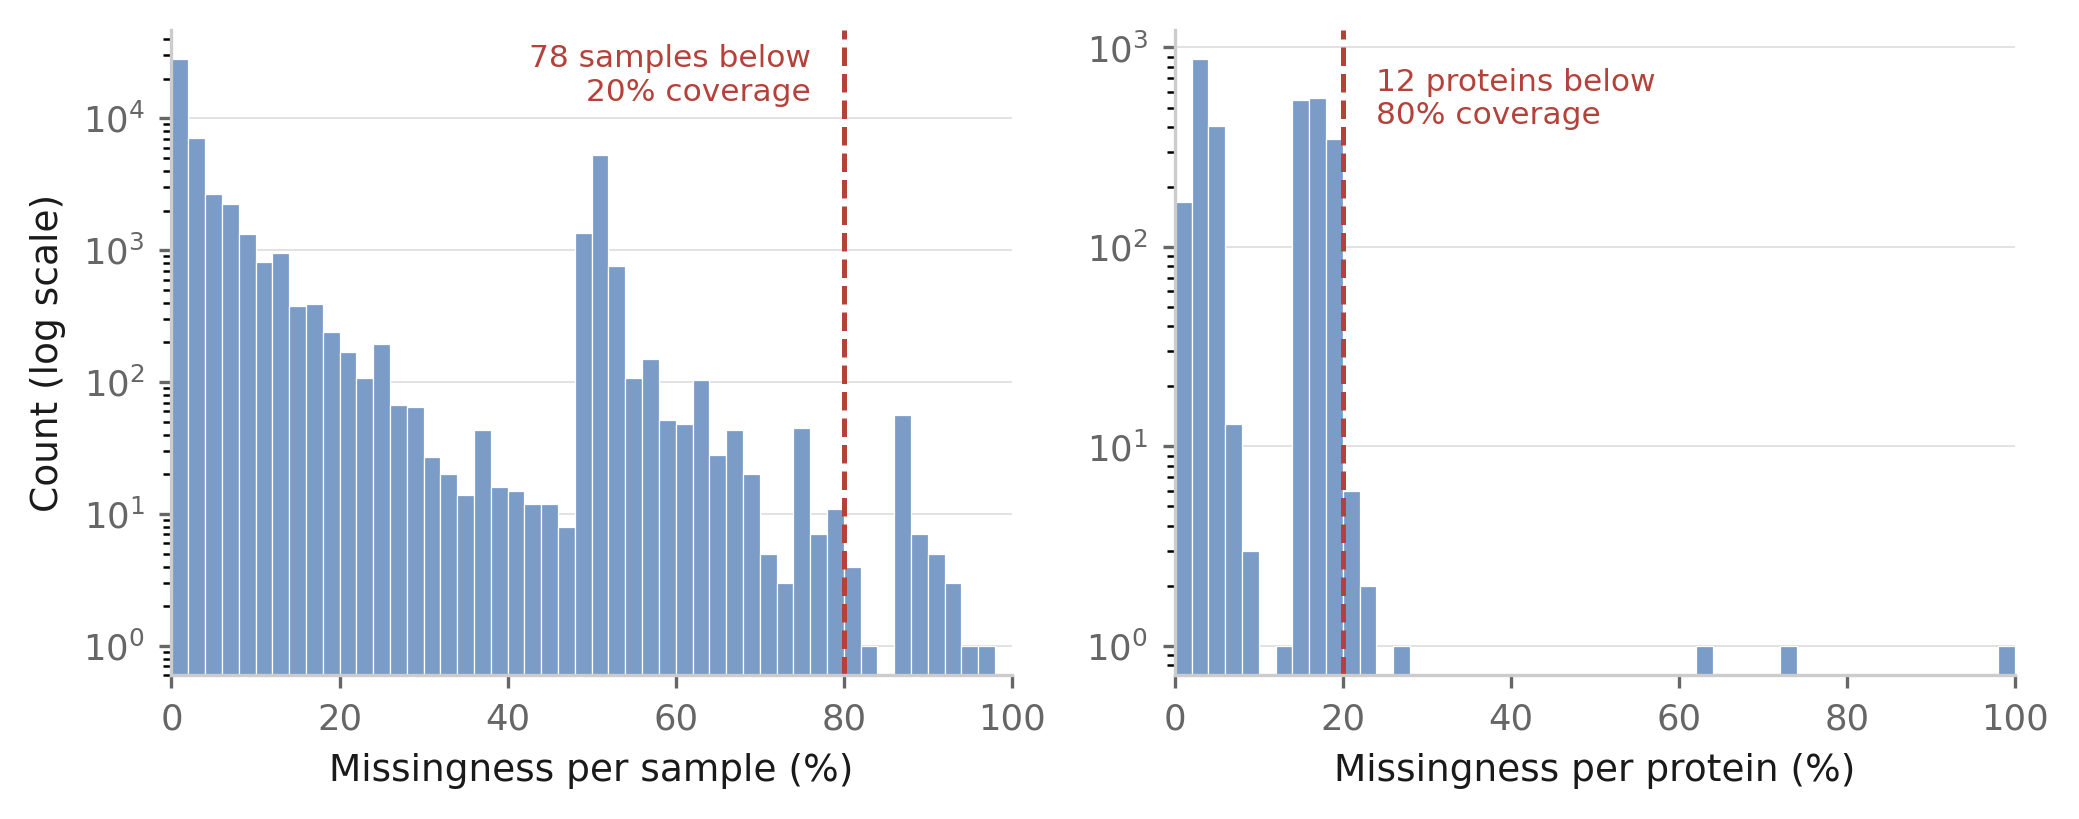
\includegraphics[width=0.95\textwidth]{figures/proteomics_missingness.png}
\caption[Missingness per sample and per protein]{Distribution of missingness per sample
(left) and per protein (right) in the UK Biobank Olink proteomics panel.}
\label{fig:proteomics-missingness}
\end{figure}


\begin{figure}[H]
\centering
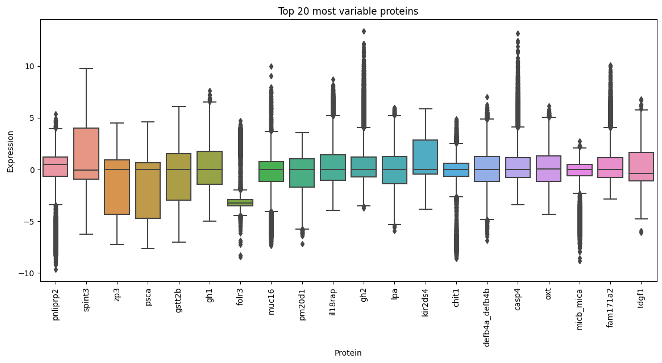
\includegraphics[width=0.85\textwidth]{figures/ukb_top20_proteins.png}
\caption[Most variable proteins]{Expression distributions of the 20 most variable proteins in the
panel. None of these falls among the 200 proteins with the highest missingness, indicating that
their variability is not an artefact of sparse measurement.}
\label{fig:top20-proteins}
\end{figure}

\subsection{Association Between Plaque Status and Proteomics}
\label{subsec:results-phase1a}

Merging the proteomics panel with the model-derived plaque phenotypes yielded 2{,}542
participants, 1{,}066 of them plaque-positive (41.9\,\%).

\paragraph{Univariate screening.}
Screening all 2{,}923 proteins individually produced 151 proteins at $p<0.05$, 37 at $p<0.01$
and 4 at $p<0.001$, with a smallest $p$-value of $5.2\times10^{-5}$ and a median $p$-value of
0.524. Under the null hypothesis, approximately 146, 29 and 3 proteins respectively would be
expected at these thresholds, so the observed counts are indistinguishable from chance. The
smallest $p$-value does not reach the Bonferroni threshold of $0.05/2923 = 1.7\times10^{-5}$,
and no protein remained significant after correction for multiple testing. Age, included in the same screen as an internal positive
control, was associated with plaque status at $p = 9.2 \times 10^{-6}$ and therefore clears the
same Bonferroni threshold that no protein reaches. The screen detects an association where one
exists; it finds none among the proteins. The strongest correlation of any single
feature with plaque status was $r = 0.088$, and that feature was age rather than a protein.

\paragraph{Multivariate classification.}
No classifier extracted usable signal from the proteomic profile
(Table~\ref{tab:phase1a-auc}). The best-performing proteomics model, gradient boosting restricted
to the 100 most informative proteins, reached a cross-validated ROC-AUC of
$0.541 \pm 0.017$; regularised logistic regression on the full panel remained at
$0.513 \pm 0.009$. All values lie close to the 0.5 expected from random classification.

\begin{table}[H]
\centering
\caption[Phase 1A classification performance]{Five-fold cross-validated ROC-AUC for predicting
model-derived plaque status from plasma proteomics ($n=2{,}542$; 2{,}923 proteins). Values are
mean $\pm$ standard deviation across folds.}
\label{tab:phase1a-auc}
\begin{tabular}{lc}
\hline
Model & ROC-AUC \\
\hline
Logistic regression (L1) & $0.508 \pm 0.011$ \\
Logistic regression (L2) & $0.513 \pm 0.009$ \\
Random forest & $0.517 \pm 0.017$ \\
XGBoost & $0.539 \pm 0.016$ \\
XGBoost, top-100 proteins & $0.541 \pm 0.017$ \\
\hline
Age and sex only & $0.551 \pm 0.028$ \\
\hline
\end{tabular}
\end{table}

\paragraph{Incremental value over demographics.}
A clinical baseline using age and sex alone reached $0.551 \pm 0.028$ and thus outperformed every
proteomics-based model. Adding proteins to this baseline did not improve discrimination but
slightly reduced it, to $0.520 \pm 0.013$ for the combination against $0.523 \pm 0.014$ for
proteins alone -- consistent with two informative variables being diluted among a hundred
uninformative ones under regularisation, rather than with any contribution from the proteome.

\paragraph{Exploratory visualisation.}
Principal component analysis of the standardised protein matrix reproduced the same picture
(Figure~\ref{fig:pca-proteomics}). The first two components capture 15.1\,\% and 4.8\,\% of the
variance. Colouring the identical embedding by age reveals a visible gradient, whereas colouring
it by plaque status shows complete overlap of the two groups. The proteomic data therefore carry
structure that these components resolve; plaque status is not part of it. As the first two
components account for only about 20\,\% of the total variance, this observation supports rather
than establishes the absence of signal.

\begin{figure}[H]
\centering
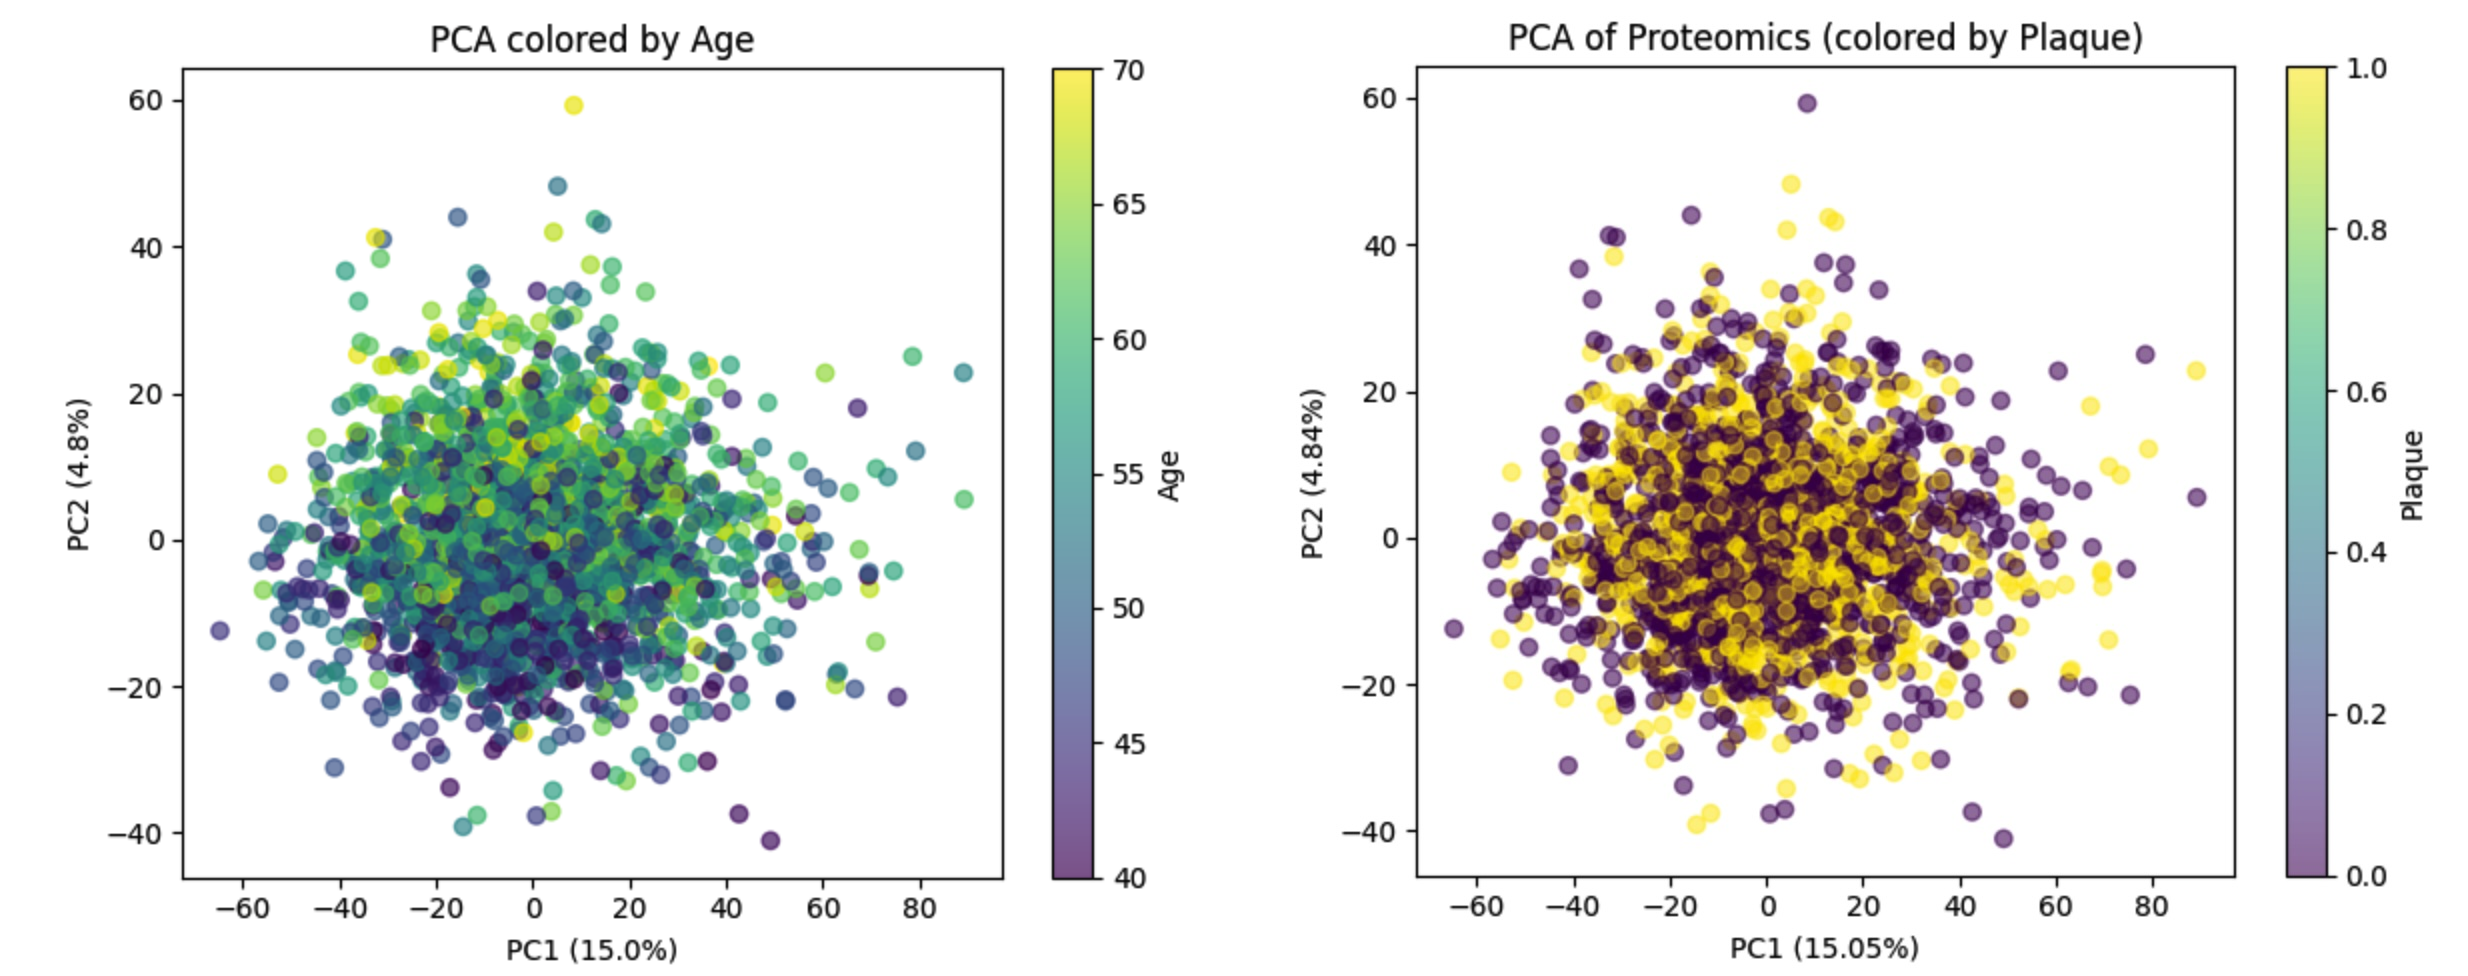
\includegraphics[width=\textwidth]{figures/pca_proteomics.png}
\caption[PCA of the proteomics panel]{Principal component analysis of the standardised protein
matrix ($n=2{,}542$). Left: coloured by age. Right: coloured by model-derived plaque status. The
same embedding separates participants by age but not by plaque status.}
\label{fig:pca-proteomics}
\end{figure}

\section{Phase 2: External Validation and Fine-Tuning}
\label{sec:results-phase2}

All results in this section use the threshold protocol of
Section~\ref{subsec:threshold-protocol}: the operating point is selected on the validation split
and applied unchanged to the 48 held-out test images.

\subsection{External Validation of the Base Model}
\label{subsec:results-external-validation}

Of the two preprocessing variants, the raw images outperformed the region-of-interest crop with
contrast equalisation on the validation split ($J = 0.493$ against $J = 0.323$), and the raw
variant was carried forward. This is consistent with the region of interest having been defined
for the UK Biobank image geometry: applied to the external images it truncates part of the
annotated plaque in 9 of the 24 plaque-positive test images, retaining as little as 64\,\% of the
annotated area in the most severe case.

On the external test set the base model reached a sensitivity of 83.3\,\% and a specificity of
62.5\,\% ($J = 0.458$). Against the 89.5\,\% and 89.2\,\% reported on its own held-out UK Biobank
test set (Section~\ref{subsec:base-model-performance}), sensitivity therefore declines by
6.2 percentage points while specificity declines by 26.7. The model continues to find plaques
that are present, but raises substantially more false alarms on plaque-free images from a source
it was not developed on.

\subsection{Performance of the Fine-Tuned Models}
\label{subsec:results-finetuned}

\begin{figure}[H]
\centering
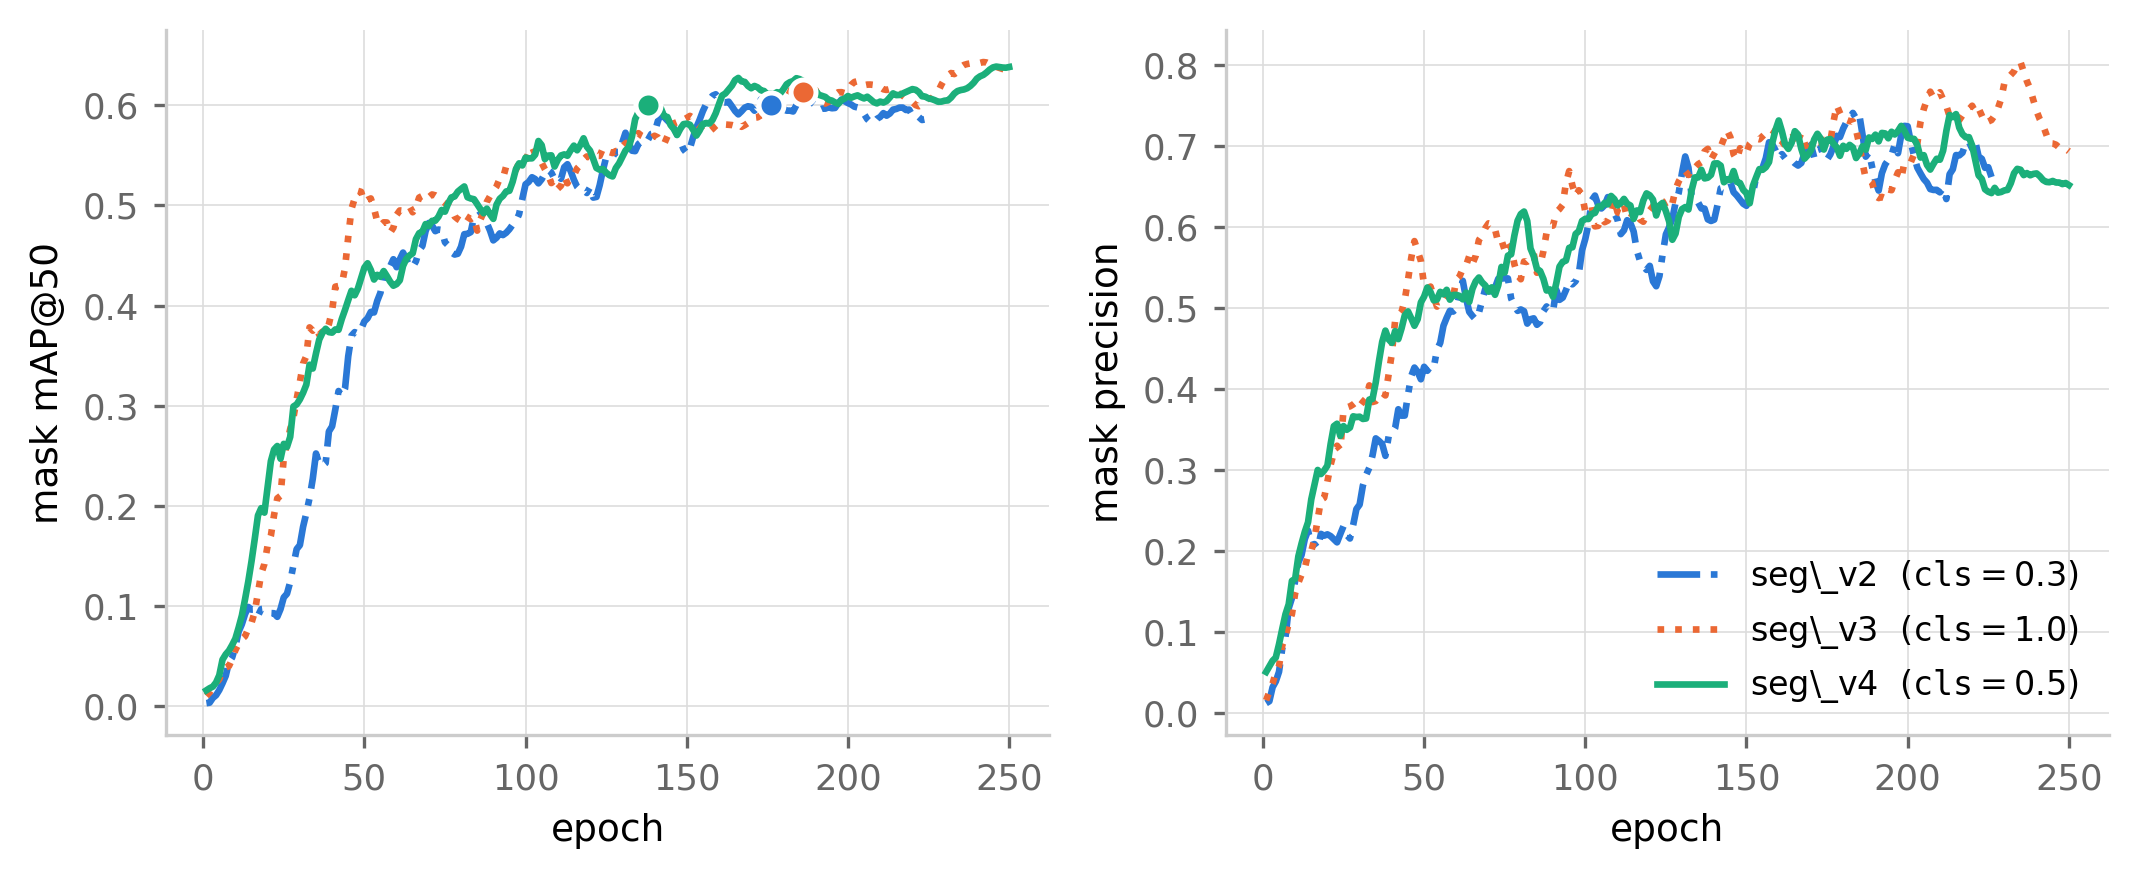
\includegraphics[width=\textwidth]{figures/cls_series.png}
\caption[Effect of the classification loss weight]{Validation mask mAP@50 (left) and mask
precision (right) over training, for the three models that differ only in the classification loss
weight. Curves are smoothed with a nine-epoch centred moving average. The marker on each curve in
the left panel gives the epoch at which that run's best checkpoint was saved, taken from the
unsmoothed values: epoch 138 for seg\_v4, 176 for seg\_v2 and 186 for seg\_v3. The higher weight
accelerates convergence and raises precision without lifting the final mAP.}
\label{fig:cls-series}
\end{figure}

On the validation split the four fine-tuned models reach a best mask mAP@50 of between 0.623 and
0.673, with seg\_v4 the strongest (Table~\ref{tab:seg-val}). On the held-out test set this
ordering does not survive: seg\_v1, seg\_v2 and seg\_v3 all reach $J = 0.625$ and differ only in
how they distribute their errors between sensitivity and specificity, while seg\_v4 -- the best
model on validation -- performs worst ($J = 0.583$).

\begin{table}[H]
\centering
\caption[Validation performance of the fine-tuned models]{Best mask mAP@50 on the validation
split, with the mask precision at the same epoch.}
\label{tab:seg-val}
\begin{tabular}{lrrr}
\hline
Model & mAP@50 (mask) & Epoch & Precision (mask) \\
\hline
seg\_v1 & 0.623 & 107 & 0.665 \\
seg\_v2 & 0.655 & 176 & 0.693 \\
seg\_v3 & 0.648 & 186 & 0.698 \\
seg\_v4 & 0.673 & 138 & 0.766 \\
\hline
\end{tabular}
\end{table}

That three models tie exactly on the test set is a consequence of its size.
Figure~\ref{fig:cls-series} shows how the classification loss weight shapes training.
 With 24
plaque-positive and 24 plaque-negative images, one image corresponds to 4.2 percentage points of
sensitivity or specificity, so differences smaller than roughly one image in each direction are
not measurable. This limitation applies to every comparison between fine-tuned variants below; it
does not apply to the comparison against the base model, where the margin is larger.

\subsection{Ensembling}
\label{subsec:results-ensembling}

Pooling the predictions of several models improves on every individual model
(Table~\ref{tab:phase2-main}, Figure~\ref{fig:roc-testset}). The combination of seg\_v1 and seg\_v2 reaches a sensitivity of
91.7\,\% at a specificity of 75.0\,\% ($J = 0.667$) with a mean Dice of 0.655. The gain is
confined to sensitivity: relative to seg\_v1 the pooled model detects one additional plaque at
unchanged specificity, while relative to seg\_v2 it detects two more at the cost of one
additional false positive. This asymmetry is structural and is examined in
Section~\ref{subsec:results-error-analysis}. Adding further models does not
help: seg\_v1\,+\,seg\_v2\,+\,seg\_v4 attains the same $J$ with higher sensitivity and lower
specificity, and the four-model combination is worse than the two-model one.

\begin{table}[H]
\centering
\caption[Phase 2 performance on the held-out test set]{Image-level performance on the 48 held-out
test images (24 plaque-positive). The threshold $t^*$ is selected on the validation split. The
final column gives the value of $J$ that would have been obtained by optimising the threshold on
the test set itself, as a measure of the optimism avoided.}
\label{tab:phase2-main}
\begin{tabular}{lrrrrrr}
\hline
Model & $t^*$ & Sens. & Spec. & $J$ & Dice & $J$ (test-optimised) \\
\hline
Base model (Omarov et al.) & 0.02 & 0.833 & 0.625 & 0.458 & -- & 0.500 \\
\hline
seg\_v1 & 0.19 & 0.875 & 0.750 & 0.625 & 0.594 & 0.708 \\
seg\_v2 & 0.18 & 0.833 & 0.792 & 0.625 & 0.576 & 0.750 \\
seg\_v3 & 0.03 & 0.792 & 0.833 & 0.625 & 0.554 & 0.750 \\
seg\_v4 & 0.22 & 0.708 & 0.875 & 0.583 & 0.502 & 0.708 \\
\hline
seg\_v1 + seg\_v2 & 0.25 & 0.917 & 0.750 & \textbf{0.667} & \textbf{0.655} & 0.792 \\
seg\_v1 + seg\_v4 & 0.25 & 0.917 & 0.708 & 0.625 & 0.619 & 0.667 \\
seg\_v2 + seg\_v4 & 0.25 & 0.833 & 0.833 & 0.667 & 0.547 & 0.708 \\
seg\_v1 + seg\_v2 + seg\_v4 & 0.25 & 0.958 & 0.708 & 0.667 & 0.655 & 0.792 \\
all four & 0.25 & 0.958 & 0.667 & 0.625 & 0.648 & 0.792 \\
\hline
\end{tabular}
\end{table}

Relative to the base model, the best configuration improves Youden's~$J$ from 0.458 to 0.667,
raising sensitivity from 83.3\,\% to 91.7\,\% and specificity from 62.5\,\% to 75.0\,\%. Roughly
half of the specificity lost to the change of data source is thereby recovered.

How much of this improvement is attributable to the segmentation formulation rather than to
adaptation to the target domain is examined by a control experiment reported in
Section~\ref{subsec:limitations-control}: a detector trained on the same data reaches the same
image-level performance as the segmentation models.

\begin{figure}[H]
\centering
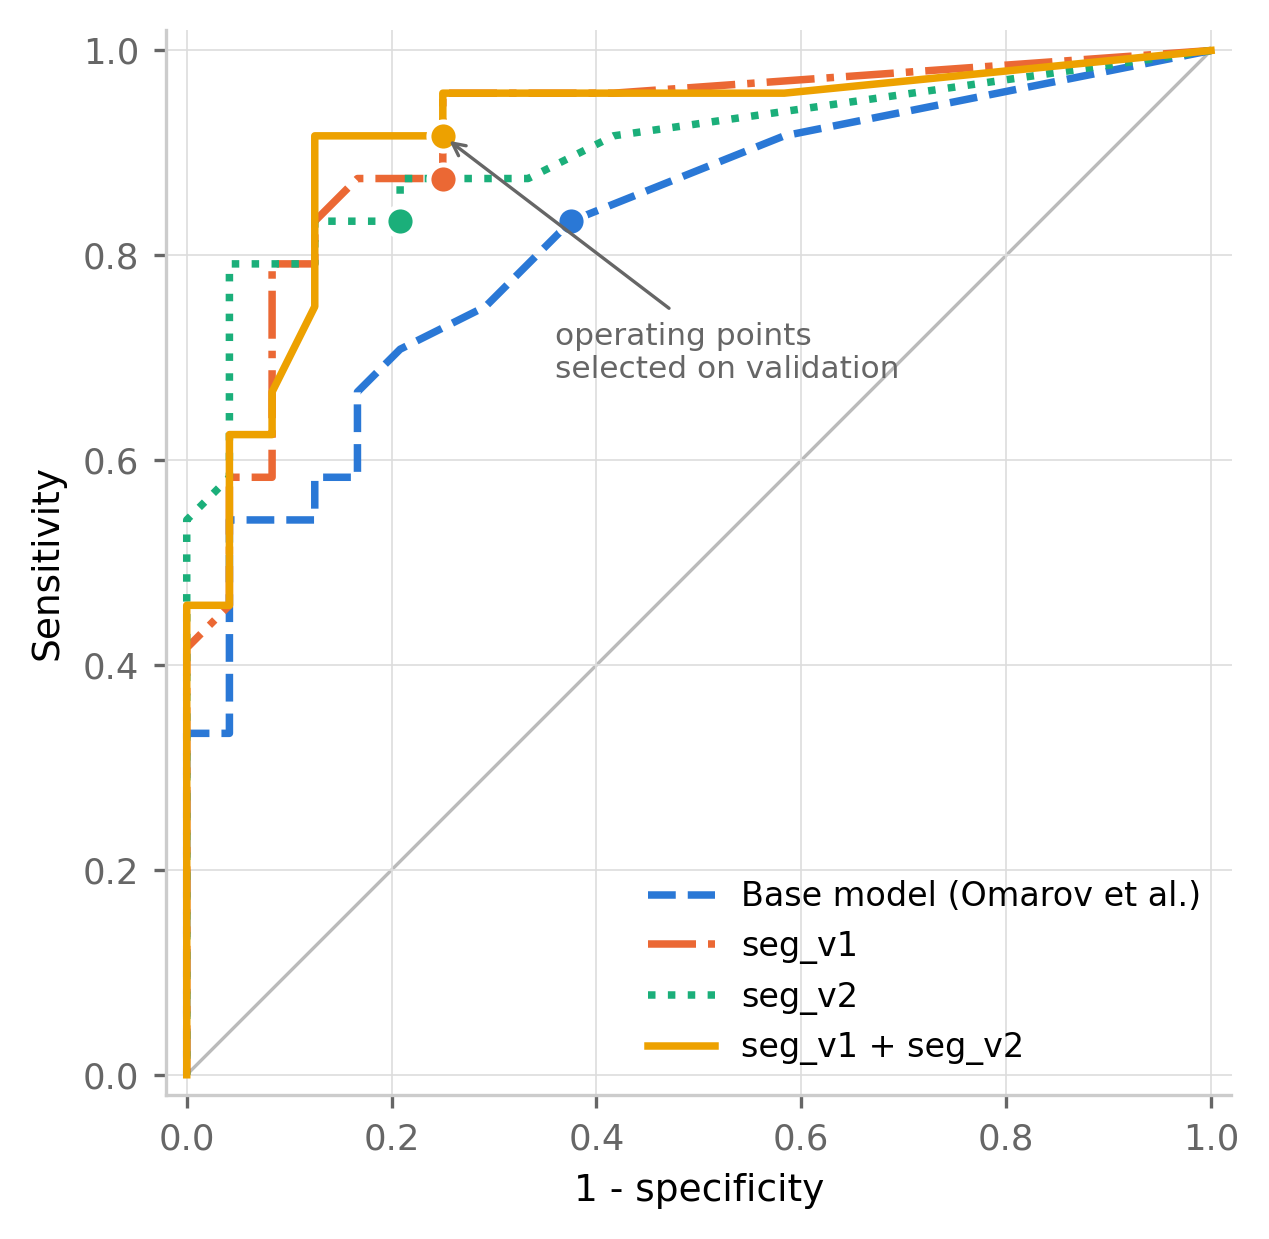
\includegraphics[width=0.62\textwidth]{figures/roc_testset.png}
\caption[Operating characteristics on the held-out test set]{Image-level operating
characteristics on the 48 held-out test images, obtained by sweeping the confidence threshold.
Markers give the operating point selected on the validation split. The base model lies below all
fine-tuned variants; pooling seg\_v1 and seg\_v2 dominates either model alone over most of the
range.}
\label{fig:roc-testset}
\end{figure}

The final column quantifies what the threshold protocol costs in reported performance. Optimising
the threshold on the test set would have raised the headline figure for seg\_v1\,+\,seg\_v2 from
0.667 to 0.792. The difference of 0.125 is of the same order as the entire improvement over the
base model, which is why the protocol matters.

\subsection{Error Analysis}
\label{subsec:results-error-analysis}

On plaque-positive images the errors of seg\_v1 and seg\_v2 are largely complementary
(Figure~\ref{fig:model-agreement}). Of the 24 plaque-positive test images, 19 are detected by
both models, two by seg\_v1 only, one by seg\_v2 only, and two by neither. Pooling therefore
recovers three images that no single model would have contributed, which is the mechanism behind
the sensitivity gain reported above.

On plaque-free images the picture is the opposite. Of the six false positives, five are shared by
both models and only one is unique. Because pooling takes the union of detections, shared false
positives cannot be removed by it, and the specificity of the pooled model is bounded by that of
its weaker constituent. This is why the improvement is confined to sensitivity, and it sets a
ceiling that no combination of these models can pass.

\begin{figure}[H]
\centering
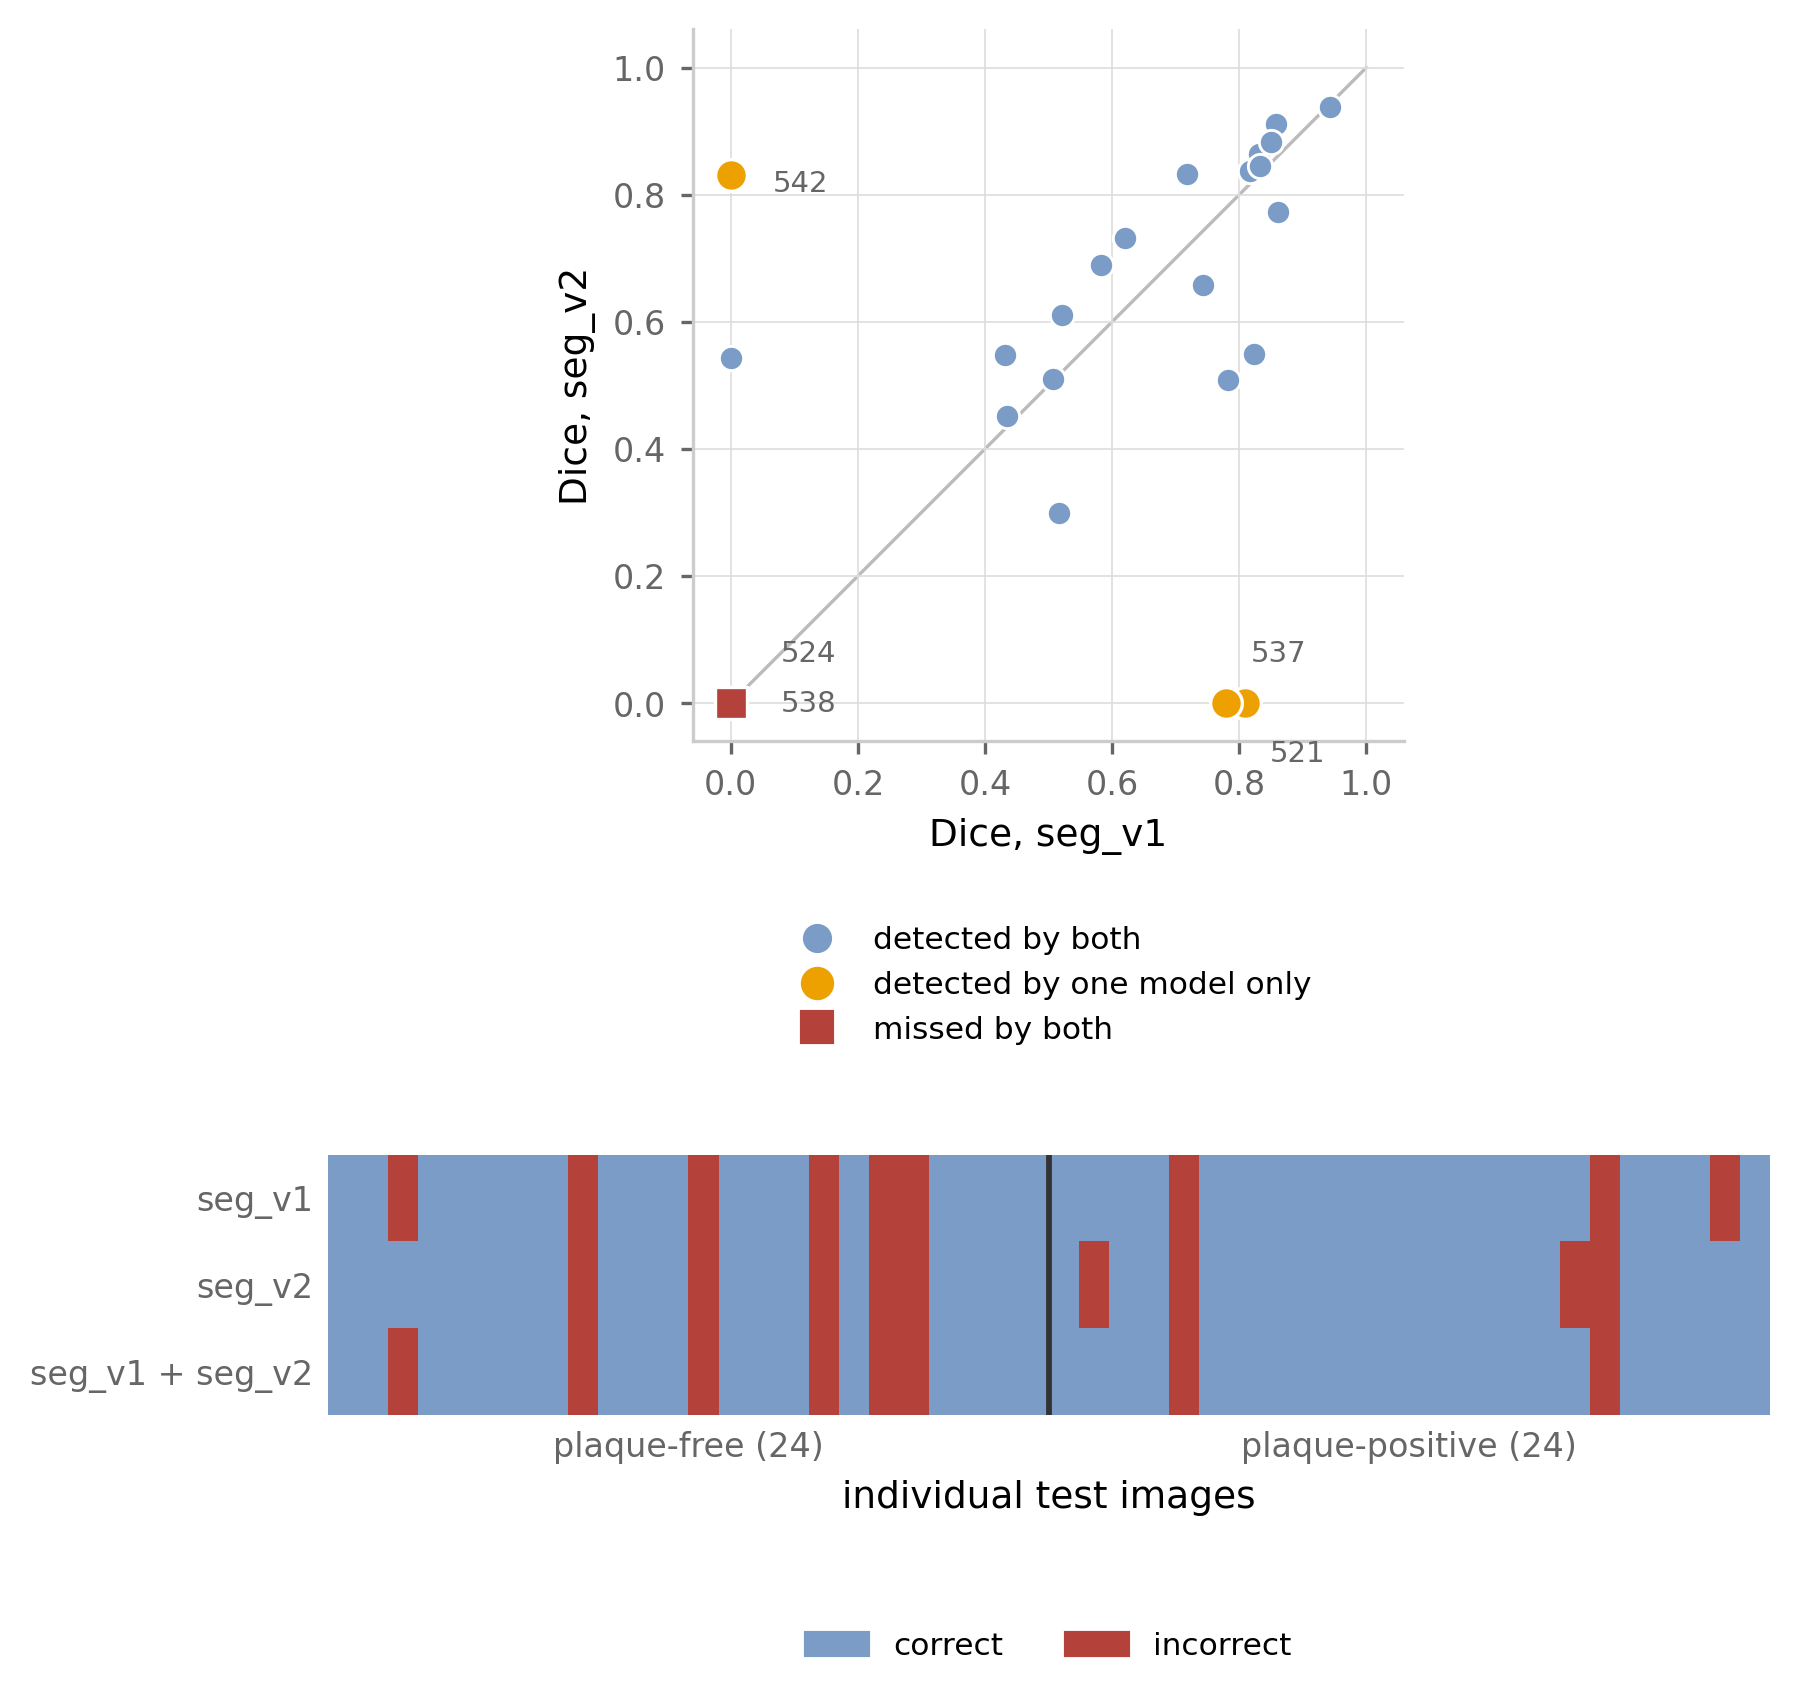
\includegraphics[width=0.72\textwidth]{figures/model_agreement.png}
\caption[Agreement between the two models]{Top: Dice coefficient of seg\_v1 against seg\_v2 for
the 24 plaque-positive test images. Bottom: per-image correctness of both models and of their
union across all 48 test images, at the operating points selected on validation. Complementarity
is present among the plaque-positive images but almost absent among the plaque-free ones.}
\label{fig:model-agreement}
\end{figure}

\subsubsection*{What the models mistake for plaque}

The shared false positives follow a single pattern (Figure~\ref{fig:false-positives}). In all six
plaque-free images that are flagged, the predicted contours follow the vessel wall over an
extended stretch rather than enclosing a focal protrusion into the lumen. Quantitatively, the
false-positive predictions are systematically thinner and smaller than true plaque annotations:
their median thickness, taken as mask area divided by bounding-box width, is 20.7 pixels against
29.9 for the annotated plaques, and their median area is 5{,}141 pixels against 9{,}705.

This is consistent with the models having learned local appearance -- a bright, elongated
structure along the wall -- rather than the diagnostic criterion itself. A plaque is defined as a
focal protrusion exceeding 50\,\% of the \emph{surrounding} intima-media thickness
(Section~\ref{subsec:external-dataset}). That criterion is relative: it requires comparing a
candidate region with the adjacent wall. A segmentation model that classifies each region on its
own appearance has no access to that comparison, and thickened but non-focal wall is precisely
the case in which the distinction matters.

\begin{figure}[H]
\centering
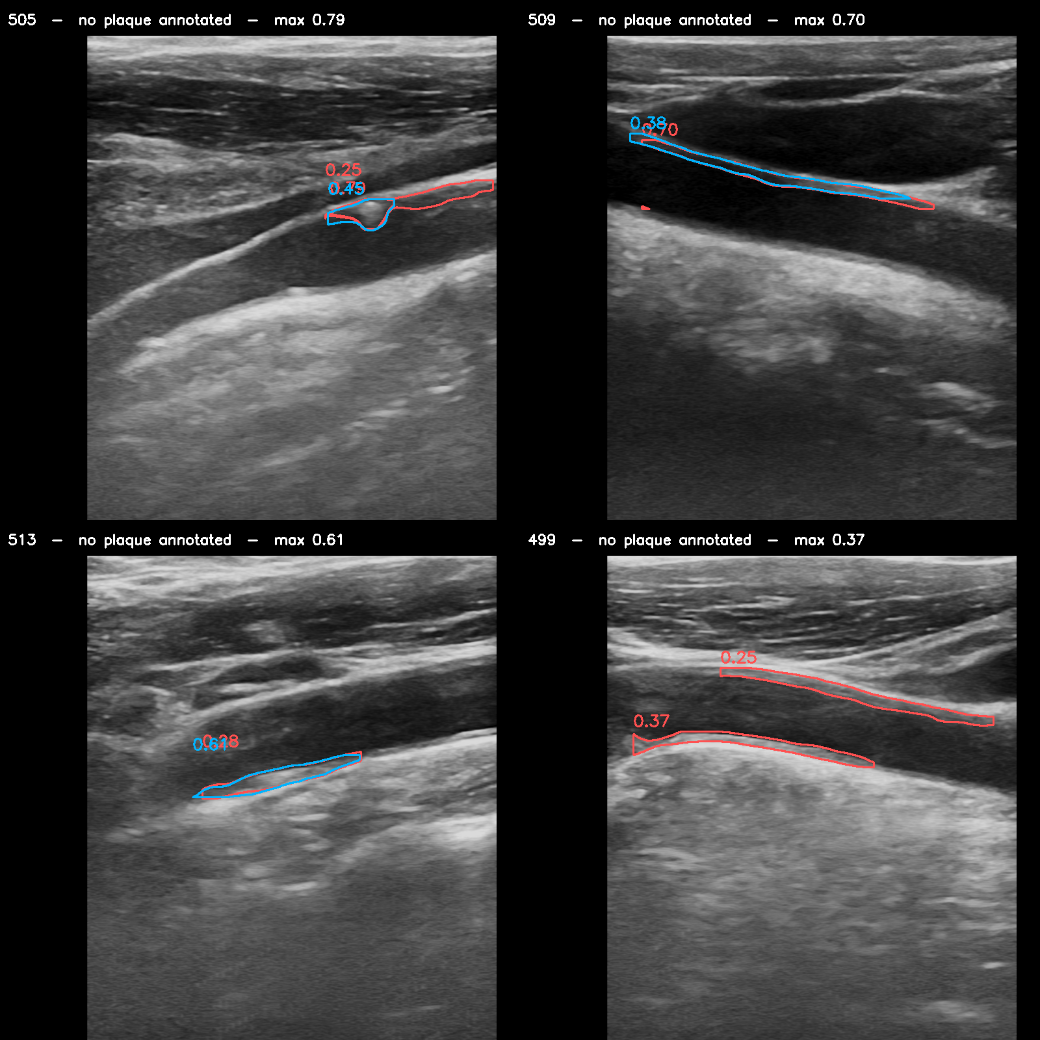
\includegraphics[width=0.78\textwidth]{figures/false_positives.png}
\caption[False positives]{Four of the six plaque-free test images that both models flag, with the
two highest-scoring contours of each model. Predictions follow the vessel wall over an extended
stretch rather than enclosing a focal protrusion.}
\label{fig:false-positives}
\end{figure}

Three candidate explanations for the residual failures were tested against the development set
and none survived. Geometry does not explain them: the mask that both models miss most severely
is at the 96th percentile of annotated area and the 90th percentile of aspect ratio, with 20
comparable instances present in the training data. Visibility does not explain them: the same
mask has a higher contrast against its surroundings than 86\,\% of training annotations. Nor does
echogenicity: the training data are evenly divided between hyperechoic and hypoechoic annotations
(157 against 159), and the difference in mean Dice between hypoechoic and hyperechoic test images
(0.580 against 0.676, on 8 and 16 images respectively) is within the noise of the sample.

\subsection{Confidence Calibration}
\label{subsec:results-calibration}

\begin{figure}[H]
\centering
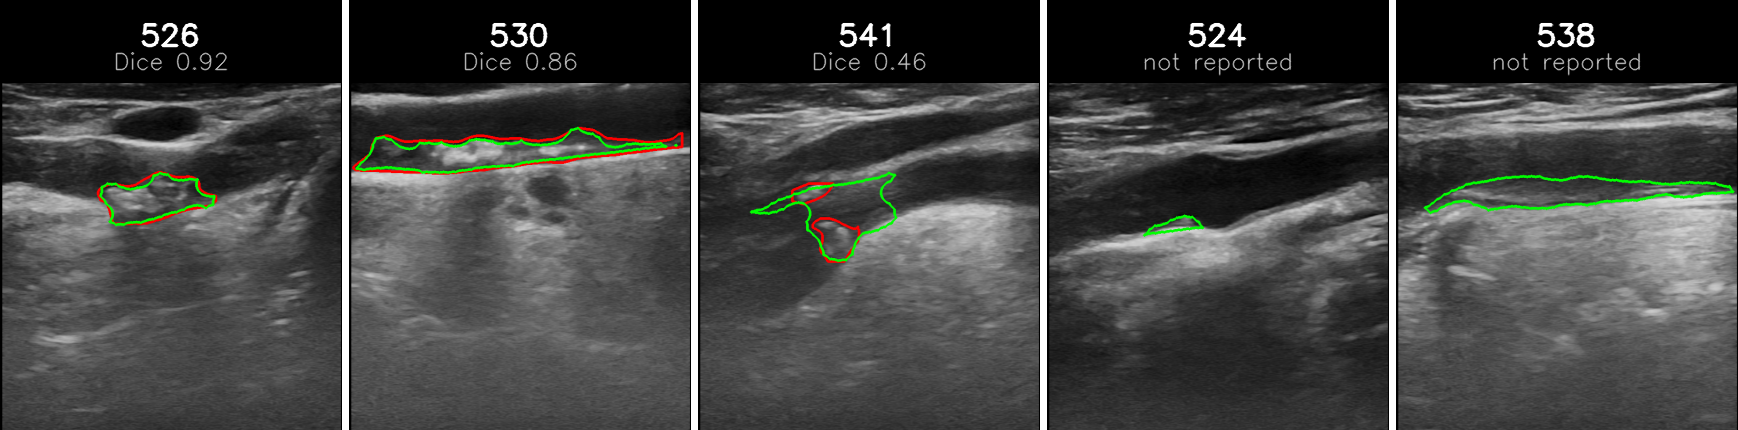
\includegraphics[width=\textwidth]{figures/qualitative_examples.png}
\caption[Qualitative examples]{Five plaque-positive test images with the annotation in green and
the pooled prediction in red, at the operating point selected on validation. The first two are
segmented accurately. The third is the only image for which no predicted instance matches the
annotation well. In the last two the models produce an accurate mask but score it far below the
threshold, so nothing is reported.}
\label{fig:qualitative}
\end{figure}

The explanation lies in the confidence scores rather than in the masks. Taking, for each
plaque-positive test image, the best-matching predicted instance irrespective of its confidence
raises the mean Dice of the seg\_v1\,+\,seg\_v2 ensemble from 0.655 to 0.794 and leaves no image
without a correct mask (Figure~\ref{fig:dice-oracle}). Both apparent failures disappear: the most severe of them is outlined at
a Dice of 0.818 by seg\_v1 and 0.789 by seg\_v2, at confidence scores of 0.0019 and 0.0010
respectively, against an operating threshold of 0.25.

The models therefore segment these plaques correctly and score them as though they were not
there. Figure~\ref{fig:qualitative} shows both behaviours alongside two successful cases. \begin{figure}[H]
\centering
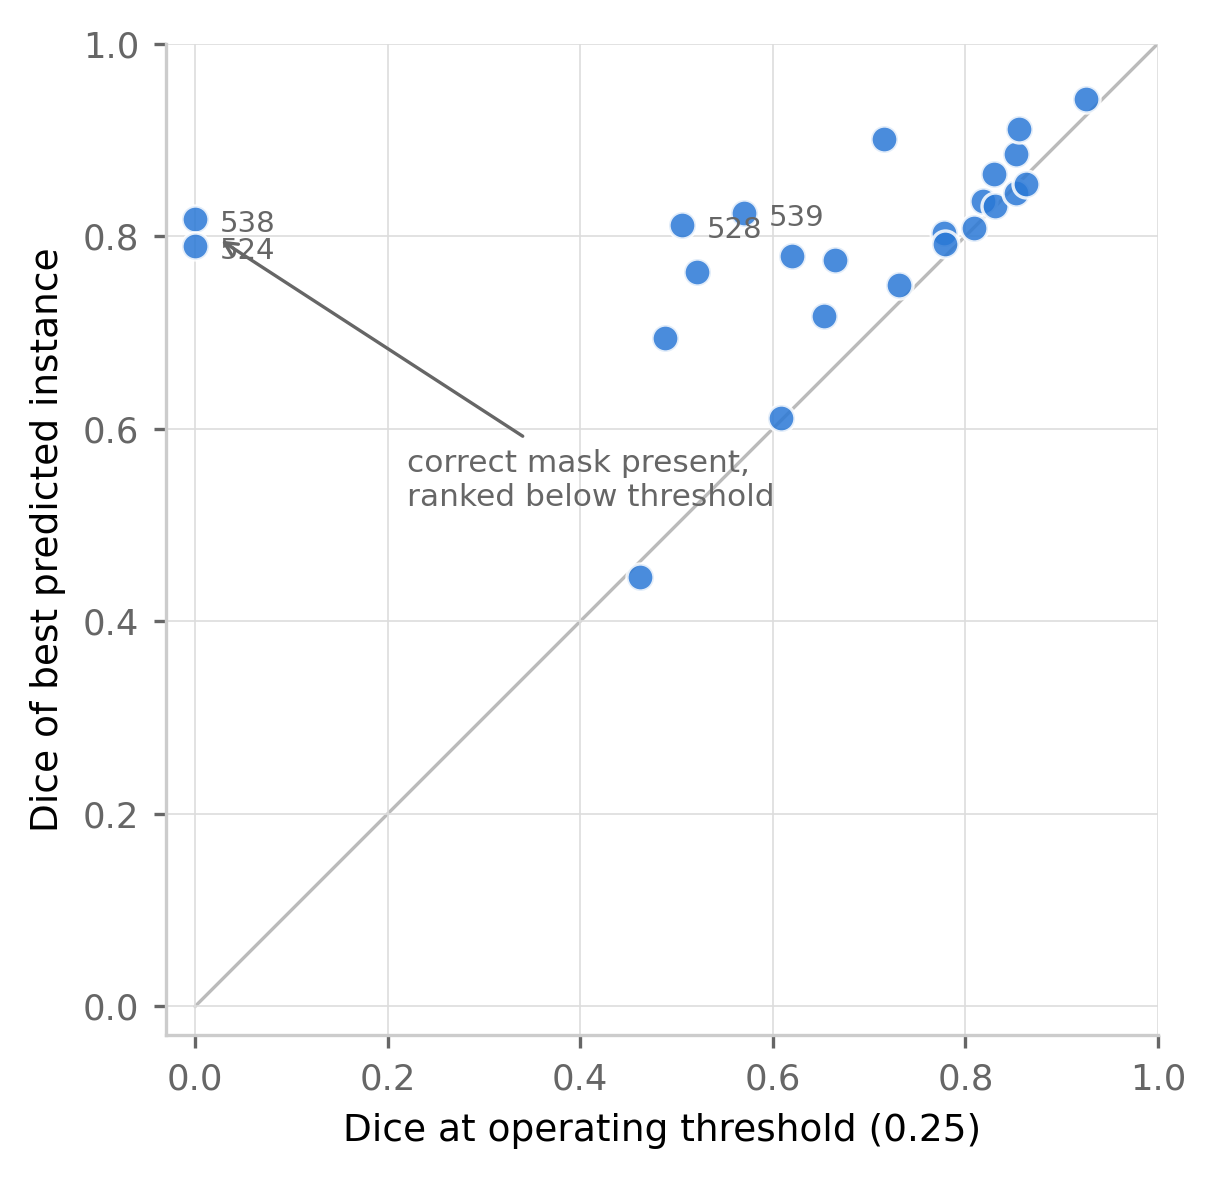
\includegraphics[width=0.58\textwidth]{figures/dice_oracle_scatter.png}
\caption[Achieved against attainable overlap]{For each of the 24 plaque-positive test images, the
Dice coefficient obtained at the operating threshold against that of the best predicted instance
irrespective of its confidence. Points on the diagonal are limited by segmentation quality; points
above it carry a correct mask that the confidence ranking discards.}
\label{fig:dice-oracle}
\end{figure}

The same pattern holds for the individual models (Table~\ref{tab:oracle}), where the gap
between the achieved and the attainable Dice is between 0.18 and 0.21.

\begin{table}[H]
\centering
\caption[Confidence-ranking analysis]{Confidence ranking against segmentation quality on the 24
plaque-positive test images. ``Dice'' is the overlap achieved by the instances the model actually
reports at its operating threshold. ``Dice (best instance)'' is the overlap of the best-matching
predicted instance irrespective of the score it carries, and therefore the ceiling that a perfect
ranking would reach; ``Gap'' is the difference between the two. ``Failures'' gives the number of
plaque-positive images in which no instance reaches the threshold, followed by the number that
would still fail if the best-matching instance were always selected -- so $4 \rightarrow 0$ means
that all four apparent misses are already segmented correctly and only the score prevents them
from being reported. ``Median confidence'' is the score carried by that best-matching instance,
taken across the 24 images.}
\label{tab:oracle}
\begin{tabular}{lrrrrr}
\hline
Model & Dice & Dice (best instance) & Gap & Failures & Median confidence \\
\hline
seg\_v1 (\texttt{cls}~=~0.3) & 0.583 & 0.769 & 0.185 & $4 \rightarrow 0$ & 0.060 \\
seg\_v2 (\texttt{cls}~=~0.3) & 0.547 & 0.754 & 0.207 & $5 \rightarrow 0$ & 0.091 \\
seg\_v3 (\texttt{cls}~=~1.0) & 0.501 & 0.680 & 0.179 & $8 \rightarrow 2$ & 0.602 \\
\hline
\end{tabular}
\end{table}

The classification loss weight controls this directly. Raising it from 0.3 to 1.0 lifts the median
confidence of the correct instance from 0.060 to 0.602, a factor of ten, confirming that the
underweighting described in Section~\ref{subsec:model-training} is the mechanism. It does so at a
cost: the attainable Dice falls from 0.769 to 0.680, and two plaque-positive images no longer
contain a correct mask at all, where seg\_v1 and seg\_v2 leave none. Optimisation pressure moves
from geometry to classification, and the masks pay for it.

The intermediate setting was therefore tested. At \texttt{cls}~=~0.5, seg\_v4 achieves the best
validation performance of all four models (Table~\ref{tab:seg-val}), including the highest mask
precision at 0.766, yet performs worst on the held-out test set. The optimum is bracketed between
0.3 and 1.0 on validation data, but the test set is too small to confirm where it lies.

\subsection{Post-hoc Re-scoring}
\label{subsec:results-rescoring}

Learned re-scoring improved the ranking of individual instances substantially and the image-level
decision not at all. The re-scorer raised the area under the curve for discriminating correct from
incorrect instances from 0.681 to 0.823 on the test set, with grouped cross-validation on the
validation split confirming the improvement (0.705 to 0.796). Applied end to end at matched
quantiles, however, Youden's~$J$ fell from 0.667 to 0.583: sensitivity rose to 100\,\%, recovering
both previously missed images, while specificity fell to 58.3\,\%.

The two objectives differ. The features available to the re-scorer describe what a plaque looks
like, which identifies genuine instances well; but in a plaque-free image the model still proposes
plaque-shaped instances, and the re-scorer promotes those equally. The original confidence,
however poorly calibrated, encodes the absence of a plaque better than any appearance-based
feature. The limiting factor for image-level performance is therefore objectness rather than
instance ranking, and it cannot be repaired after training.

\section{Effect of the Duplicate Images}
\label{sec:results-duplicates}

Four plaque-positive test images are byte-identical to images in the development partition of
the published split (Section~\ref{subsec:duplicates}) and were therefore seen during training.
The partition was used as distributed; the overlap is a property of the dataset rather than of
the split applied here. Excluding the four images leaves
20 plaque-positive and 24 plaque-negative images and lowers the figures of the best configuration
as follows.

\begin{table}[H]
\centering
\caption[Performance with and without the duplicated images]{seg\_v1\,+\,seg\_v2 at the operating
point selected on validation, computed on the full test partition and with the four duplicated
images removed.}
\label{tab:dedup}
\begin{tabular}{lrrrrr}
\hline
& $n_{\text{pos}}$ & Sens. & Spec. & $J$ & Dice \\
\hline
Full test partition & 24 & 0.917 & 0.750 & 0.667 & 0.655 \\
Duplicates excluded & 20 & 0.900 & 0.750 & 0.650 & 0.615 \\
\hline
\end{tabular}
\end{table}

\begin{figure}[H]
\centering
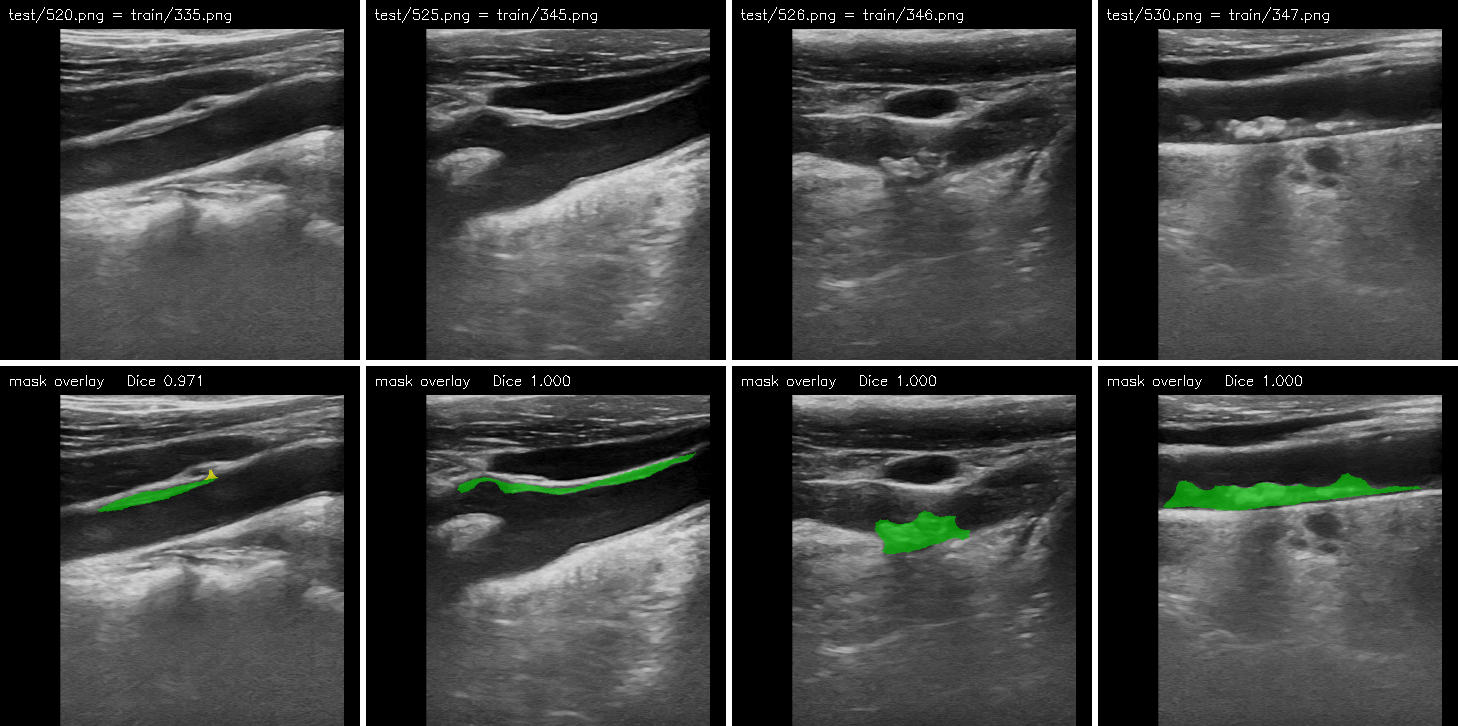
\includegraphics[width=\textwidth]{figures/duplicate_pairs.png}
\caption[Images duplicated across the published split]{The four images appearing in both
partitions of the published split. Top row: the shared image. Bottom row: the two annotations
overlaid -- green where they agree, yellow where only the test-partition mask covers a pixel, red
where only the development-partition mask does. Three pairs carry byte-identical masks. The
first, \texttt{520.png}, was annotated twice independently; the two masks agree at a Dice
coefficient of 0.971, the difference being confined to the distal tip of the lesion.}
\label{fig:duplicate-pairs}
\end{figure}

The four pairs are shown in Figure~\ref{fig:duplicate-pairs}.

The four affected images are among those the model handles best, with Dice coefficients between
0.82 and 0.92, which is consistent with their having been seen in training. The effect on the
aggregate is nonetheless small: Youden's $J$ falls by 0.017 and the mean Dice by 0.040, against a
margin over the base model of 0.192 on the deduplicated set. The deduplicated figures are the
ones this thesis relies on; both are reported so that the comparison with other work using the
published split remains possible.
